\documentclass[]{article}
\title{SA4E - Übung 3}
\author{Marlin Zapp}
\pdfminorversion=6

\usepackage[outputdir=output]{minted} % for code snippets
\usepackage[T1]{fontenc}
\usepackage[ngerman]{babel}
\usepackage{csquotes}
\usepackage{svg}
\usepackage[font={small},hang,labelfont=bf]{caption}
\usepackage{hyperref} % has autoref
\usepackage{pdfpages}
\usepackage{color}
\usepackage[dvipsnames,svgnames,table]{xcolor}
\usepackage{fancyhdr}

%bib
\usepackage[
style=apa,
backend=biber,
maxcitenames=1,
maxbibnames=999
]{biblatex}
\addbibresource{quellen.bib}

\begin{document}
\maketitle

In dieser Übung geht es darum, das Spiel \emph{Ave Caesar} so zu implementieren, dass alle Spielbrett-Segmente einzelne Programme sind, die miteinander über eine Streaming-Architektur kommunizieren.

\tableofcontents

\section{Spielprinzip}
\label{sec:spielprinzip}

Das Grundprinzip von \emph{Ave Caesar} ist, dass $n$ Spieler versuchen, jeweils zuerst drei Runden eines Wagenrennens über einen Parcours zu beenden. Auf dem Weg muss jeder Spieler mindestens einmal auf einem vordefinierten Feld stehen bleiben, um Caesar zu grüßen. Jeder Spieler muss, falls möglich, bei seinem Zug eine seiner drei Karten spielen und anschließend nachziehen oder ansonsten aussetzen. Die Karten haben Werte von 1-6, um jene Anzahl an Feldern vorwärts zu ziehen.

\section{Implementierung}
\label{sec:implementierung}

Die Implementierung des Spiels erfolgt in mehreren Schritten. Zunächst wird mithilfe des Skripts \texttt{generate-circular-course.py} ein Parcours in Form einer JSON-Datei generiert. Der Parcours ist in mehrere Segmente aufgeteilt. Ein weiteres Skript, \texttt{run.py}, startet die einzelnen Segmente als Instanzen des Skripts \texttt{segment.py} und gibt ihnen mit, auf welche Weise sie miteinander verbunden sind.

\subsection{Parcours-Generierung}
\label{subsec:parcours-generierung}

Der Parcours wird mithilfe von zwei Parametern generiert:
\begin{itemize}
    \item \texttt{num\_tracks}: Die Anzahl der Spuren, auf denen die Spieler fahren.
    \item \texttt{num\_segments}: Die Anzahl der Segmente, aus denen jede Spur besteht.
\end{itemize}
Grundsätzlich besteht ein normaler Spur-Abschnitt aus einem Segment \texttt{segment-<i>-<j>} für jede Spur. Dabei steht $i$ für die Spur und $j$ für den Abschnitt. Allerdings gibt es zwei Sonderfälle:
\begin{itemize}
    \item Im $0$-ten Abschnitt befindet sich ein zusätzliches Segment \texttt{segment-<num\_tracks+1>-0}, auf dem nach Runde 1, 2 oder 3 Caesar gegrüßt werden muss.
    \item Abschnitte des Typs \emph{bottleneck} sind Engstellen. Hier existiert nur das Segment \texttt{segment-0-<j>}, während alle anderen Spuren in diesem Abschnitt kein Segment besitzen.
\end{itemize}
Die Parcours-Generierung definiert abhängig vom aktuellen und nächsten Segment-Typ, welche Segmente auf ein bestimmtes Segment folgen. Dies wird in der JSON-Datei als \texttt{nextSegments} definiert. Wenn zum Beispiel zwei Abschnitte vom Typ \emph{wall-divided} aufeinander folgen, dann ist kein Spurwechsel möglich und jedes \texttt{segment-<i>-<j>} hat ein Array \texttt{nextSegments} der Länge 1 mit \texttt{segment-<i>-<j+1>} als einzigem Eintrag. \autoref{fig:parcours} versucht, die verfügbaren Segment-Typen anschaulich zu machen.
\begin{figure}
    \caption{Die Graphik veranschaulicht den Beispiel-Parcours, der in der \texttt{parcours.json} zu finden ist, um einen Eindruck für die drei verschiedenen Segment-Typen zu geben. In diesem Parcours würden drei Spieler spielen. Die möglichen Züge sind über die \texttt{nextSegments} in der \texttt{parcours.json} nachvollziehbar.}
    \label{fig:parcours}
    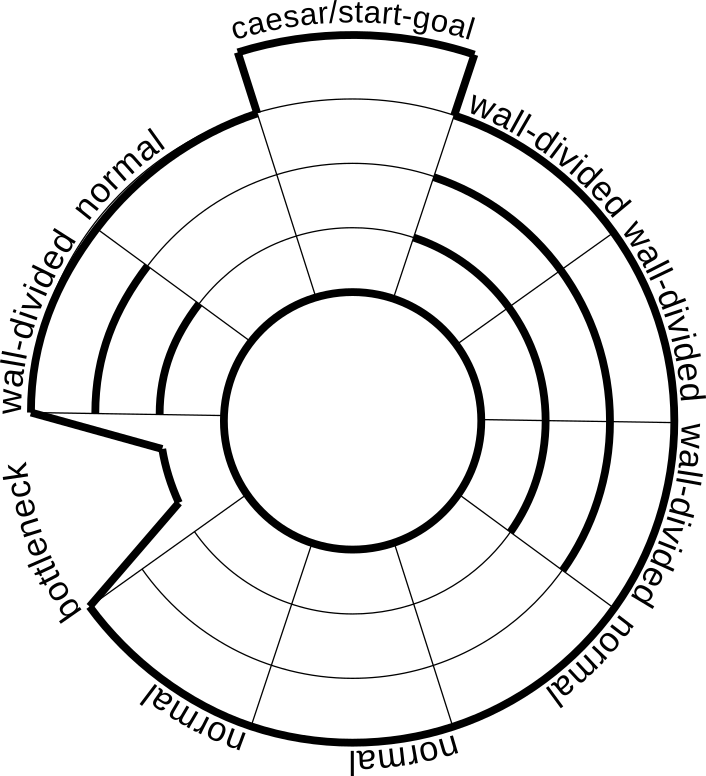
\includegraphics[width=\textwidth]{parcours.png}
\end{figure}

\subsection{Initialisierung}
\label{subsec:initialisierung}

Damit die Kommunikation zwischen den Segmenten funktioniert, müssen drei Apache Kafka Server-Instanzen auf den Ports \texttt{29092}, \texttt{39092} und \texttt{49092} laufen. Diese werden über die \texttt{compose.yaml} definiert, welche einfach ein Beispiel für ein Kafka Cluster aus dem \href{https://github.com/apache/kafka/blob/trunk/docker/examples/docker-compose-files/cluster/combined/plaintext/docker-compose.yml}{Kafka Github Repository} ist. Die Server-Instanzen können mit \texttt{docker compose up} gestartet werden.\par
In \texttt{run.py} wird für jedes Segment aus der JSON-Datei, die den Parcours enthält, ein Prozess mit dem Skript \texttt{segment.py} gestartet. Für jedes der \texttt{<num\_tracks>} Start-Segmente wird dann ein Spieler mit drei Karten initialisiert.
\begin{minted}{python}
player = {
    "player_id": segment_id.split("-")[-2],
    "round": 0,
    "has_greeted_caesar": False,
    "cards": cards,
}
\end{minted}
Jedes Segment besitzt einen Apache Kafka Consumer und einen Apache Kafka Producer und kommuniziert darüber mit anderen Segmenten. Der Consumer und Producer verbindet sich jeweils mit den drei Server-Instanzen. Um das Spiel zu starten, werden die Spielerinformationen in einem \emph{start}-Event an die Start-Segmente geschickt. Dabei gibt es einen großen Delay zwischen den Initialisierungs-Nachrichten, damit die Spieler ungefähr der Reihe nach am Zug sind.

\subsection{Felder erkunden}
\label{subsec:scouting}

Sobald ein Spieler am Zug ist, wird von dem Segment, auf dem er sich befindet, erkundet, auf welches Feld er mit seinen drei Karten am besten gehen sollte. Die Suche erfolgt mithilfe von \emph{scout}- und \emph{scout-result}-Nachrichten, die in einer Tiefensuche von Segment zu Segment geschickt werden. Dabei tragen die Nachrichten unter anderem die Information, welche Segmente bereits erkundet wurden und welche potentiellen Ziel-Segmente gefunden wurden. An Segmenten, die bereits belegt sind, endet die Suche.

\subsection{Bewegung}
\label{subsec:move}

Nach der Erkundung werden die Ziel-Segmente verglichen. Das \emph{Caesar}-Segment wird bevorzugt, ansonsten wird die größt-mögliche Karte gespielt. Eine \emph{move}-Nachricht wird an das Ziel-Segment geschickt und die Spieler-Informationen werden aktualisiert. In dem Zuge wird mithilfe der Information, welcher Pfad genommen wurde, auch überprüft, ob der Spieler eine Runde vollendet hat und das Spiel mit oder ohne Caesar-Gruß beendet hat.

\section{Fazit}
\label{sec:conclusion}

Das Aufsetzen der Apache Kafka Container war sehr simpel, die Muster-Datei für ein Server-Cluster aus drei Instanzen hat direkt funktioniert. Die Kommunikation über Apache Kafka in der Implementierung war sehr intiutiv. Man konnte die üblichen Verfahren der nachrichtenbasierten Kommunikation problemlos anwenden und das Producer-Consumer-Konzept war für die Aufgabe gut geeignet.\par
In der vorliegenden Implementierung kann es zu Fehlern kommen, wenn Spieler gleichzeitig spielen, da die Bestimmung von besetzten Feldern nicht isoliert abläuft. Als zukünftige Aufgabe könnte man die Implementierung verbessern, indem die Reihenfolge der Spieler nicht über ein Delay geregelt wird, sondern über eine sequentielle Abfolge von Spielzügen. Dann könnten keine Probleme mehr auftreten.\par
Ein Problem der Implementierung ist, dass die Züge sehr lange dauern, da die Sequentialisierung annähernd über ein Delay erreicht wird. Außerdem ist die Zugdauer so lange, da in der Tiefensuche nach einem passenden Feld Nachrichten von vielen Producern zu vielen Consumern gesendet werden müssen. Jedes Segment in der Reichweite der Karte sendet mindestens eine Nachricht. Dies ist jedoch dem Anwendungsbeispiel geschuldet, da Streaming-Architekturen natürlich nicht für die Implementierung von Spiel-Logik gedacht sind.

\end{document}
